\documentclass[a4paper,12pt]{article} 

% packages and main settings
\usepackage[left=3cm, right=2cm, top=2cm, bottom=2cm]{geometry}
\usepackage[english]{babel}    
\usepackage[utf8]{inputenc}  
\usepackage[T1]{fontenc}        
\usepackage{lmodern}            
\usepackage{microtype}          
\usepackage{amsmath}
\usepackage{amsfonts, amsthm, amssymb, graphicx, booktabs}
\usepackage{bm} %bold epsilon
\usepackage{newclude}   
\usepackage{placeins}  %surpresses floating tables
\usepackage[labelfont=bf]{caption} %Figure etc steht dann in small caps 
\usepackage[labelsep=period]{caption} % dot after figure, table caption.
\usepackage[flushleft]{threeparttable} % for notes below table
\usepackage{multirow} % for table cell merge along rows
\usepackage{graphicx} % to adjust tablesize to textwidth
\usepackage{caption}  % for centered captions
\usepackage{float} % to set of autopositioning of tables
\usepackage[bottom,hang,flushmargin]{footmisc} % forces footnotes to the bottom
\usepackage{setspace}           % Fuer 1.5 fachen Zeilenabstand  
\onehalfspacing % 1.5 cm Zeilenabstand
%Bibtex
\usepackage[round,sort&compress]{natbib}

\bibliographystyle{chicago} % chicago bib style like in AER
\usepackage[hidelinks]{hyperref} % fuer links und verweise. Cleverref ist eigentlich besser. 


% Create header. The header must be surpressed for 
% every first page per section and a solution
% for the Appendix is used in the respective subfile.
\usepackage{fancyhdr}
\pagestyle{fancy}
\fancyhf{}
\chead{\nouppercase{\textit{\leftmark}}}
\cfoot{\thepage}
\renewcommand{\headrulewidth}{0pt} % no vertical line

%\usepackage{lipsum}  % check if formats work

\usepackage{afterpage} %clearpage w/o pagebreak for "header bug"

% Expectation symbol
\DeclareMathOperator*{\E}{\mathbb{E}}

% thin space, limits underneath in displays
% for strike through
\DeclareMathOperator*{\argmax}{argmax}
\newcommand*{\defeq}{\stackrel{\text{def}}{=}}
\usepackage[normalem]{ulem}
% try to use strikeout in section headers and others
\DeclareRobustCommand{\hsout}[1]{\texorpdfstring{\sout{#1}}{#1}}

% for gray table row color
\usepackage[table]{xcolor}

% decimal dot alignment in table columns
\usepackage{siunitx}

% for footnotes in table
\usepackage[flushleft]{threeparttable}

% for underbar
\newcommand{\ubar}[1]{\text{\b{$#1$}}}

\usepackage{tikz}

% Setup for urls
\usepackage{url}

\defcitealias{Respy-Stenzel.2019}{\textit{respy}}
\defcitealias{Gabler.2019}{\textit{estimagic}}
\defcitealias{Stenzel.2020}{\textit{Master's Thesis Replication Repository}}
\defcitealias{NLSY79}{NLSY79}


\usepackage{tikz}
\begin{document}

\newpage % delete after section is complete

\section{EE method}
\begin{align} \label{eq:EE}
d_i^{(j)} =  \frac{Y(\bold{X_{\sim i}^{(j)}}, X_i^{(j)} + \Delta^{(i,j)})}{\Delta^{(i,j)}},
\end{align}

\begin{align}
\mu_i = \frac{1}{r} \sum_{j=1}^{r} d_i^{(j)}.
\end{align}


\begin{align}
\sigma_i = \frac{1}{r} \sum_{j=1}^{r} (d_i^{(j)} - \mu_i)
\end{align}


\begin{align}
\mu_i^* = \frac{1}{r} \sum_{j=1}^{r} \big| d_i^{(j)} \big|.
\end{align}

\begin{align}
\mu_{i,\sigma}^* = \mu_i^* \frac{\sigma_{X_i}}{\sigma_Y}.
\end{align}

Scaling provides link from "deterministic effect" to impact on variation of Y. Parameters may have large effects on Y but not on its variation: The impact of $X$ may be strong but always the same if $\sigma_x=\epsilon$.  Especially tricky, if Y does also not vary a lot.

Example: linear function with two parameters: high coeff - low SD and low coeff, high SD.

\newpage


\section{Sampling schemes}

One EE per parameter per subsample.

\begin{align}
\underset{(k+1)\times k}{\bold{R}} =
\begin{pmatrix}
a_1 & a_2 & ... & a_k \\
\bold{b_1} & a_2 & ... & a_k \\
a_1 & \bold{b_2} & ... & a_k \\
\vdots & \vdots & 	\ddots & \vdots\\
a_1 & a_2 & ... & \bold{b_k}
\end{pmatrix}
\end{align}
\noindent
Contains choice of (quasi-random) sequence. Implies share of very high steps.

\begin{align}
\underset{(k+1)\times k}{\bold{T}} =
\begin{pmatrix}
a_1 & a_2 & ... & a_k \\
\bold{b_1} & a_2 & ... & a_k \\
\bold{b_1} & \bold{b_2} & ... & a_k \\
\vdots & \vdots & 	\ddots & \vdots\\
\bold{b_1} & \bold{b_2} & ... & \bold{b_k}
\end{pmatrix}
\end{align}\newpage
Contains choice of two numerical parameters. Lower bound of step is 0.5 given step function.

\section{EE method for correlated inputs}


	\begin{enumerate}
	\item $\bold{z} = \pmb{\Phi^{-1}({u})}$
	\item $\bold{z_c} = \bold{Q^T z^T}$
	\item $\bold{x} = \pmb{\mu} + \bold{z_c(i)}\pmb{\sigma(i)}$
	\end{enumerate}

Transform samples. $N(3k+1)$ and $3Nk$ function evals.


Correlations include step.

\begin{align} \label{eq:t1_min}
\mathcal{T}_1(\bold{T_{i+1,*}}; i-1)
=
\begin{pmatrix}
a_k & a_1 & ... & ... &  a_{k-1} \\
\bold{b_1} & a_2 & ... & ... &  a_k \\
\bold{b_2} & a_3 & ... & ... &  \bold{b_1} \\
\vdots & \vdots & \vdots & 	\ddots &  \vdots\\
\bold{b_k} & \bold{b_{1}} & ... & ... &  \bold{b_{k-1}}
\end{pmatrix}
\end{align}
\begin{align} \label{eq:t1_sub}
\mathcal{T}_1(\bold{T_{i,*}}; i-1)=
\begin{pmatrix}
a_1 & a_2 & ... & ... &  a_k \\
a_2 & ... & ... &  a_k & \bold{b_1} \\
a_3 & ... & ... &  \bold{b_1} & \bold{b_2} & \\
\vdots & \vdots & \vdots & 	\ddots &  \vdots\\
\bold{b_1} & \bold{b_{2}} & ... & ... &  \bold{b_{k}}
\end{pmatrix}
\end{align}

Correlations exclude step.

\begin{align}
\mathcal{T}_1(\bold{T_{i,*}}; i-1)=
\begin{pmatrix}
a_2 & a_3 & ... & ... &  a_1 \\
a_3 & ... & a_k &  \bold{b_1} & a_2 \\
a_4 & ... & \bold{b_1} &  \bold{b_2} & a_3 & \\
\vdots & \vdots & \vdots & 	\ddots &  \vdots\\
\bold{b_2} & \bold{b_{3}} & ... & ... &  \bold{b_{1}}
\end{pmatrix}
\end{align}

\newpage
Trajectory design only.

Activates distortions by numerical parameters and general differences in drawing the elements between schemes.

\begin{align} \label{eq:d_full}
d_i^{full,T} = \frac{f\big(\mathcal{T}(\bold{T_{i+1,*}}; i-1)\big) - f\big(\mathcal{T}(\bold{T_{i,*}}; i)\big)}{\Delta}.
\end{align}


\begin{align} \label{eq:d_ind}
d_i^{ind, T} = \frac{f\big(\mathcal{T}(\bold{T_{i+1,*}}; i)\big) - f\big(\mathcal{T}(\bold{T_{i,*}}; i)\big)}{\Delta}.
\end{align}

\newpage
Improvements. Denominator can be written much simpler as $\mathcal{T}(b_i) - \mathcal{T}(a_i)$.

\begin{align}
d_i^{c,T} = \frac{f\big(\mathcal{T}(\bold{T_{i+1,*}}; i-1)\big) - f\big(\mathcal{T}(\bold{T_{i-1,*}}; i)\big)}{F^{-1}\big(\Phi^u(b_i)\big) - F^{-1}\big( \Phi^u(a_i)\big)}
\end{align}

\begin{align} \label{eq:u1}
d_i^{u, T} = \frac{f\big(\mathcal{T}(\bold{T_{i+1,*}}; i)\big) - f\big(\mathcal{T}(\bold{T_{i,*}}; i)\big)}{F^{-1}\big({Q^T}_{k,*k-1}(j)T_{i+1,*k-1}^T(j) + {Q^T}_{k,k} \Phi^u(b_i)\big) - F^{-1}\big({Q^T}_{k,*k-1}(j)T_{i,*k-1}^T(j)+{Q^T}_{k,k} \Phi^u(a_i)\big)}
\end{align}
\newpage

\section{Replication and Validation}

Linear function with three parameters and Correlations equal to 0.9, 0.4, 0.01.
Numerical parameter lead to re-lineariation of measures in GM'17.\\


Let $f(X_1, ..., X_k)$ = $\sum_{i = 1}^{k} c_i X_i$ be an arbitrary linear function. Let $\rho_{i,j}$ be the linear correlation between $X_i$ and $X_j$. Then, for all $i \in 1, ..., k$, I expect:\footnote{These results correspond to the intuition provided by the example in \cite{Saltelli.2008}, p. 123.}
\begin{align}
d_i^{u,*} = c_i \label{eq:diu}\\
d_i^{c,*} = \sum_{j = 1}^{k} \rho_{i,j} c_{j}. \label{eq:dic}.
\end{align}
Both equations state that, conceptually, the result does not depend on the sampling scheme.
\newpage


\setlength{\tabcolsep}{12pt} %from 6
\begin{table}[H]
	\centering
	\caption{Replication and validation - trajectory design}
	\label{tab:repval1}
	\renewcommand{\arraystretch}{1.2}%
	\begin{threeparttable}
		\begin{tabular}{cS[table-format=3.2]S[table-format=3.2]S[table-format=3.2]S[table-format=3.2]}
			\toprule
			{Measure}     & {GM'17}   & {Repl. $\mu^{*}$}\tnote{$\dagger$} & {Repl. $\sigma$}\tnote{$\ddagger$} & {S'20} \\ \midrule
			
			
			& 1.20  & 1.36         & 0.83         & 1.00 \\
			\qquad $\mu^{*,ind}$                               & 1.30  & 1.48         & 0.91         & 1.00 \\
			& 3.20  & 3.11         & 1.94         & 1.00 \\
			&&&& \\
			& 0.55  & 0.00         & 0.56         & 0.00 \\
			\qquad $\sigma^{ind}$                            & 0.60  & 0.00         & 0.62         & 0.00 \\
			& 1.30  & 0.00         & 1.32         & 0.00 \\
			&&&& \\
			& 14.90 & 16.20        & 9.97         & 2.30 \\
			\qquad $\mu^{*,full}$                              & 12.50 & 13.45        & 8.31         & 1.91 \\
			& 10.00 & 9.93         & 6.18         & 1.41 \\
			&&&& \\
			& 6.50  & 0.00         & 6.74         & 0.00 \\
			\qquad $\sigma^{full}$                           & 5.50  & 0.00         & 5.63         & 0.00 \\
			& 4.00  & 0.00         & 4.20         & 0.00 \\		
			\bottomrule	
		\end{tabular}
		\begin{tablenotes}
			
			\item[$\dagger$] \footnotesize $0^{num}=0.00001$ and $l=4$. 
			\item[$\ddagger$] $0^{num}=0.00000001$ and $l=24$.\par
			
		\end{tablenotes}
	\end{threeparttable}
\end{table}
\hspace{1cm} %linebreak.
% Please add the following required packages to your document preamble:
% \usepackage{booktabs}
\setlength{\tabcolsep}{12pt} %from 6
\begin{table}[H]
	\centering
	\caption{Replication and validation - radial design}
	\label{tab:repval2}
	\renewcommand{\arraystretch}{1.2}%
	\begin{tabular}{cS[table-format=3.2]S[table-format=3.2]S[table-format=3.2]}
		\toprule
		{Measure}     & {GM'17}   & {Replication}  & {S'20} \\ 
		\midrule
		
		& 0.60  & 0.57         &  1.00 \\
		\qquad $\mu^{*,ind}$                               & 0.75  & 0.85         &  1.00 \\
		& 1.50  & 1.31         &  1.00 \\
		&&& \\
		& 0.20   & 0.10         &  0.00 \\
		\qquad $\sigma^{ind}$                            & 0.30   & 0.41         &  0.00 \\
		& 0.85  & 0.22         & 0.00 \\
		&&& \\
		& 7.50  & 6.84         &  2.30 \\
		\qquad $\mu^{*,full}$                              & 6.80   & 7.77         &  1.91 \\
		& 4.75  & 4.19         &  1.41 \\
		&&& \\
		& 2.90  & 1.15         &  0.00 \\
		\qquad $\sigma^{full}$                           & 2.65  & 3.68         &  0.00 \\
		& 2.50   & 0.70         &  0.00 \\ \bottomrule
	\end{tabular}
\end{table}
\newpage
\begin{figure}[H]
	\caption{Grid points in standard normal sample space for trajectory design with $l=4$}
	\centering
	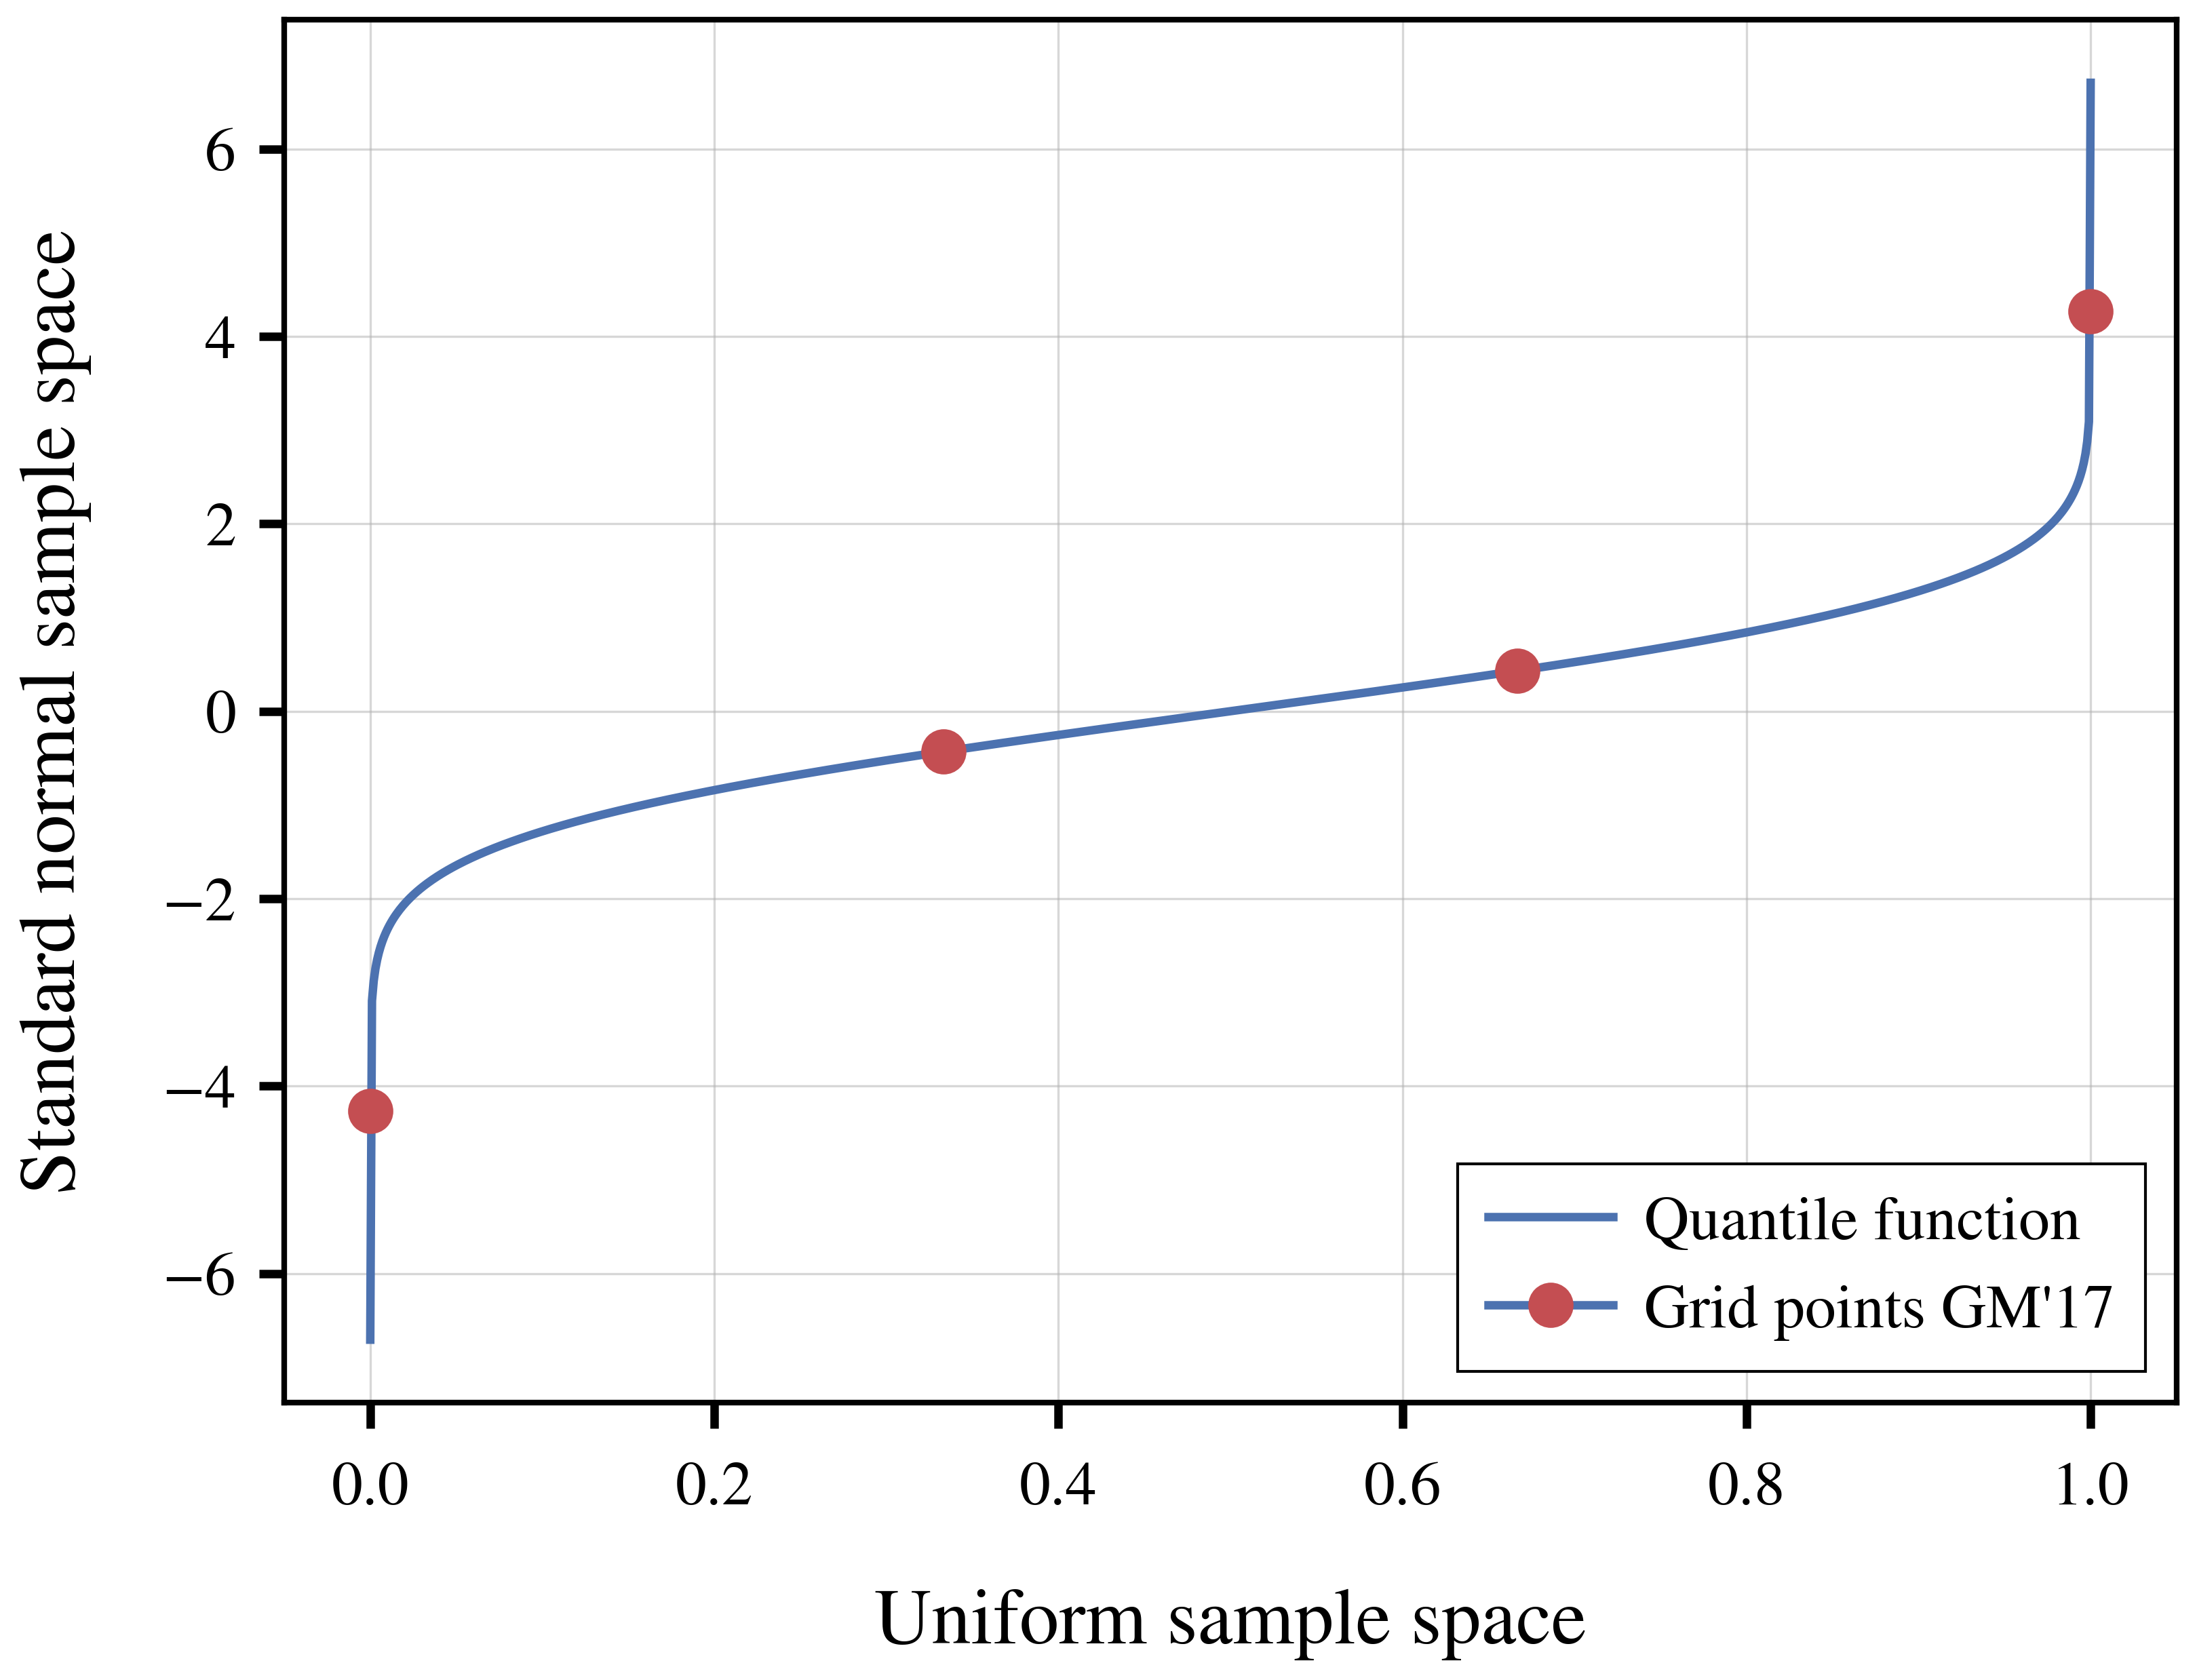
\includegraphics[scale=0.40]{../../../scrypy/figures/quantile_fct}
	\label{fig:invcdf}
\end{figure}

\newpage
\section{Results: Uncertainty Analysis}

\begin{figure}[H]
	\caption{Probability distribution of quantity of interest $q$}
	\centering
	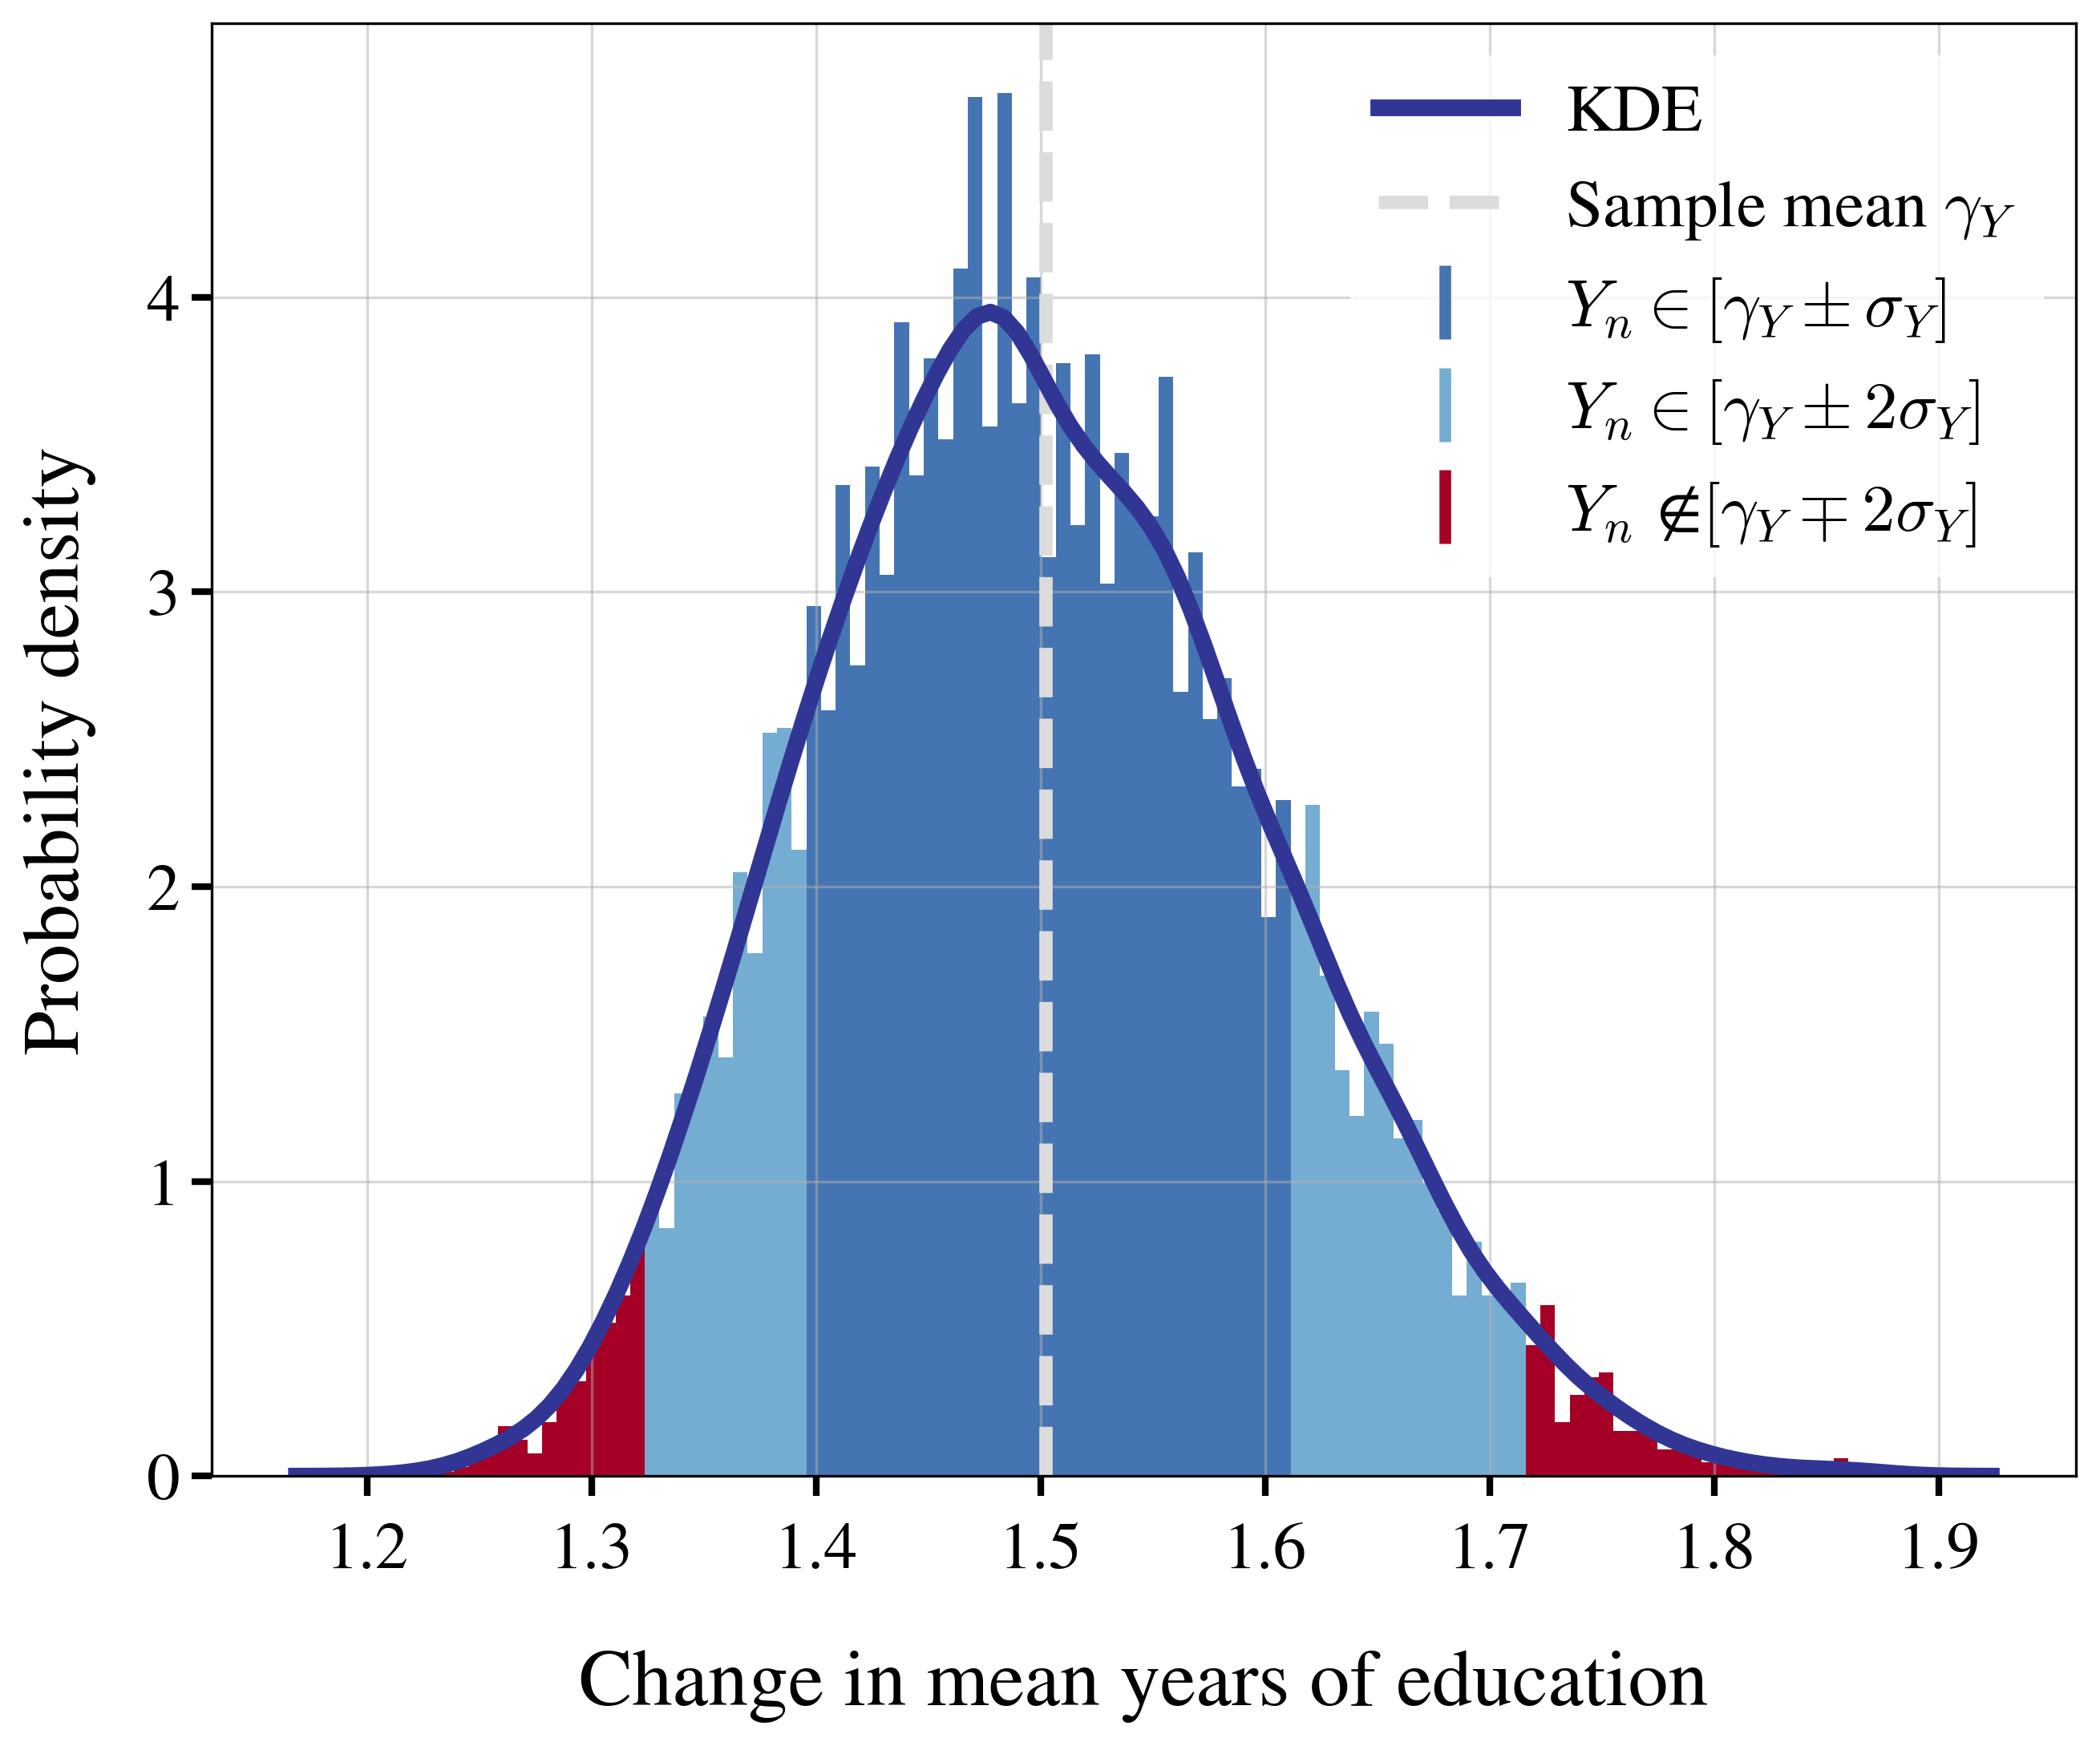
\includegraphics[scale=0.7]{../../../scrypy/figures/distplot}
	\label{fig:dist}
\end{figure}

\begin{figure}[H]
	\caption{Comparison of shares of occupation decision over time between scenarios with cone plots}
	\centering
	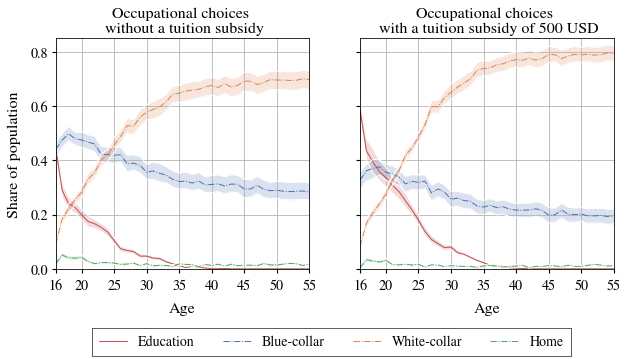
\includegraphics[scale=0.75]{../../../scrypy/figures/cone_plot_choice_shares}
	\label{fig:paths}
\end{figure}



\newpage
\subsection{Results: Qualitative Sensitivity Analysis}
Be cautious!
\newpage
\setlength{\tabcolsep}{22pt} %from 6
\begin{table}[H] 
	\centering
	\begin{threeparttable}
		\caption[Model Parametrization]{Mean absolute correlated and uncorrelated elementary effects\\ (based on 150 subsamples in trajectory and radial design)}
		\label{tab:params}
		\renewcommand{\arraystretch}{1.2}%
		\begin{tabular}{cS[table-format=3.2]S[table-format=3.2]@{\hskip 0.7in}|@{\hskip 0.5in}S[table-format=3.2]S[table-format=3.2]}

			{Parameter}     & {$\mu^{*,c}_T$}   & {$\mu^{*,c}_R$} & {$\mu^{*,u}_T$} & {$\mu^{*,u}_R$}\\ \midrule
			\textit{General} \\
			$\delta$ & 17   & 23 & 476 & 415   \\    \midrule
			\textit{Blue-collar}\\    
			$\beta^b$ & 1   & 3            & 43 & 88    \\
			$\beta_e^b$ & 11  &    14        & 406  & 443    \\
			$\beta^b_b$ & 25  & 51            & 688  & 1169    \\
			$\beta^b_{bb}$ & 871 & 934           & 15540  & 17860     \\
			$\beta^b_w$ & 29    & 48             & 73  &  143  \\
			$\beta^b_{ww}$ & 389    & 460           & 869 &  1183    \\ \midrule
			\textit{White-collar}\\
			$\beta^w$ & 1   & 3            & 50 &  117   \\
			$\beta^w_e$ & 26   & 28          & 943 &  852    \\
			$\beta^w_w$ & 24  & 47            & 718 &  1521   \\
			$\beta^w_{ww}$ & 933  & 997           & 12257 & 18069   \\
			$\beta^w_b$ & 131 & 127           & 309 &  356   \\
			$\beta^w_{bb}$ & 120 & 1352         & 2088 &  2477   \\ \midrule
			\textit{Education} \\
			$\beta^e$     & 0.0008    & 0.0002              & 0.001&  0.003   \\
			$\beta_{he}^e$     & 0.0001    & 0.0002              & 0.001  & 0.001    \\
			$\beta_{re}^e$     & 0.0003   & 0.0002               & 0.0003  &   0.0006  \\ \midrule
			\textit{Home} \\
			$\beta^h$    & 0.0003  & 0.0003                 & 0.00002  & 0.00002     \\ \midrule
			\multicolumn{4}{l}{\textit{Lower Triangular Cholesky Matrix}} \\
			$c_{1}$      & 8    & 16             & 18 &  37   \\
			$c_{2}$      & 8   & 11             & 22 & 24   \\
			$c_{3}$      & 0.0004   & 0.0004             & 0.0004 & 0.0007    \\
			$c_{4}$      & 0.0004    & 0.00008              & 0.0002 & 0.0003    \\
			$c_{1,2}$     & 4   & 4            & 10 &  10  \\
			$c_{1,3}$      & 0.0005   & 0.0006              & 0.0006 &  0.0005   \\
			$c_{2,3}$      & 0.0003    & 0.0005             &  0.0006 &   0.001 \\
			$c_{1,4}$      & 0.00004    & 0.00005            &   0.0004 &  0.0005 \\
			$c_{2,4}$      & 0.0001    & 0.0002           & 0.0001  &  0.0002  \\
			$c_{3,4}$      & 0.0001   & 0.0001                & 0.00008  &  0.0001   \\ \bottomrule
		\end{tabular}
	\end{threeparttable}
\end{table}
\newpage
\begin{figure}[H]
	\caption{Sigma-normalized mean absolute Elementary Effects for trajectory design}
	\centering
	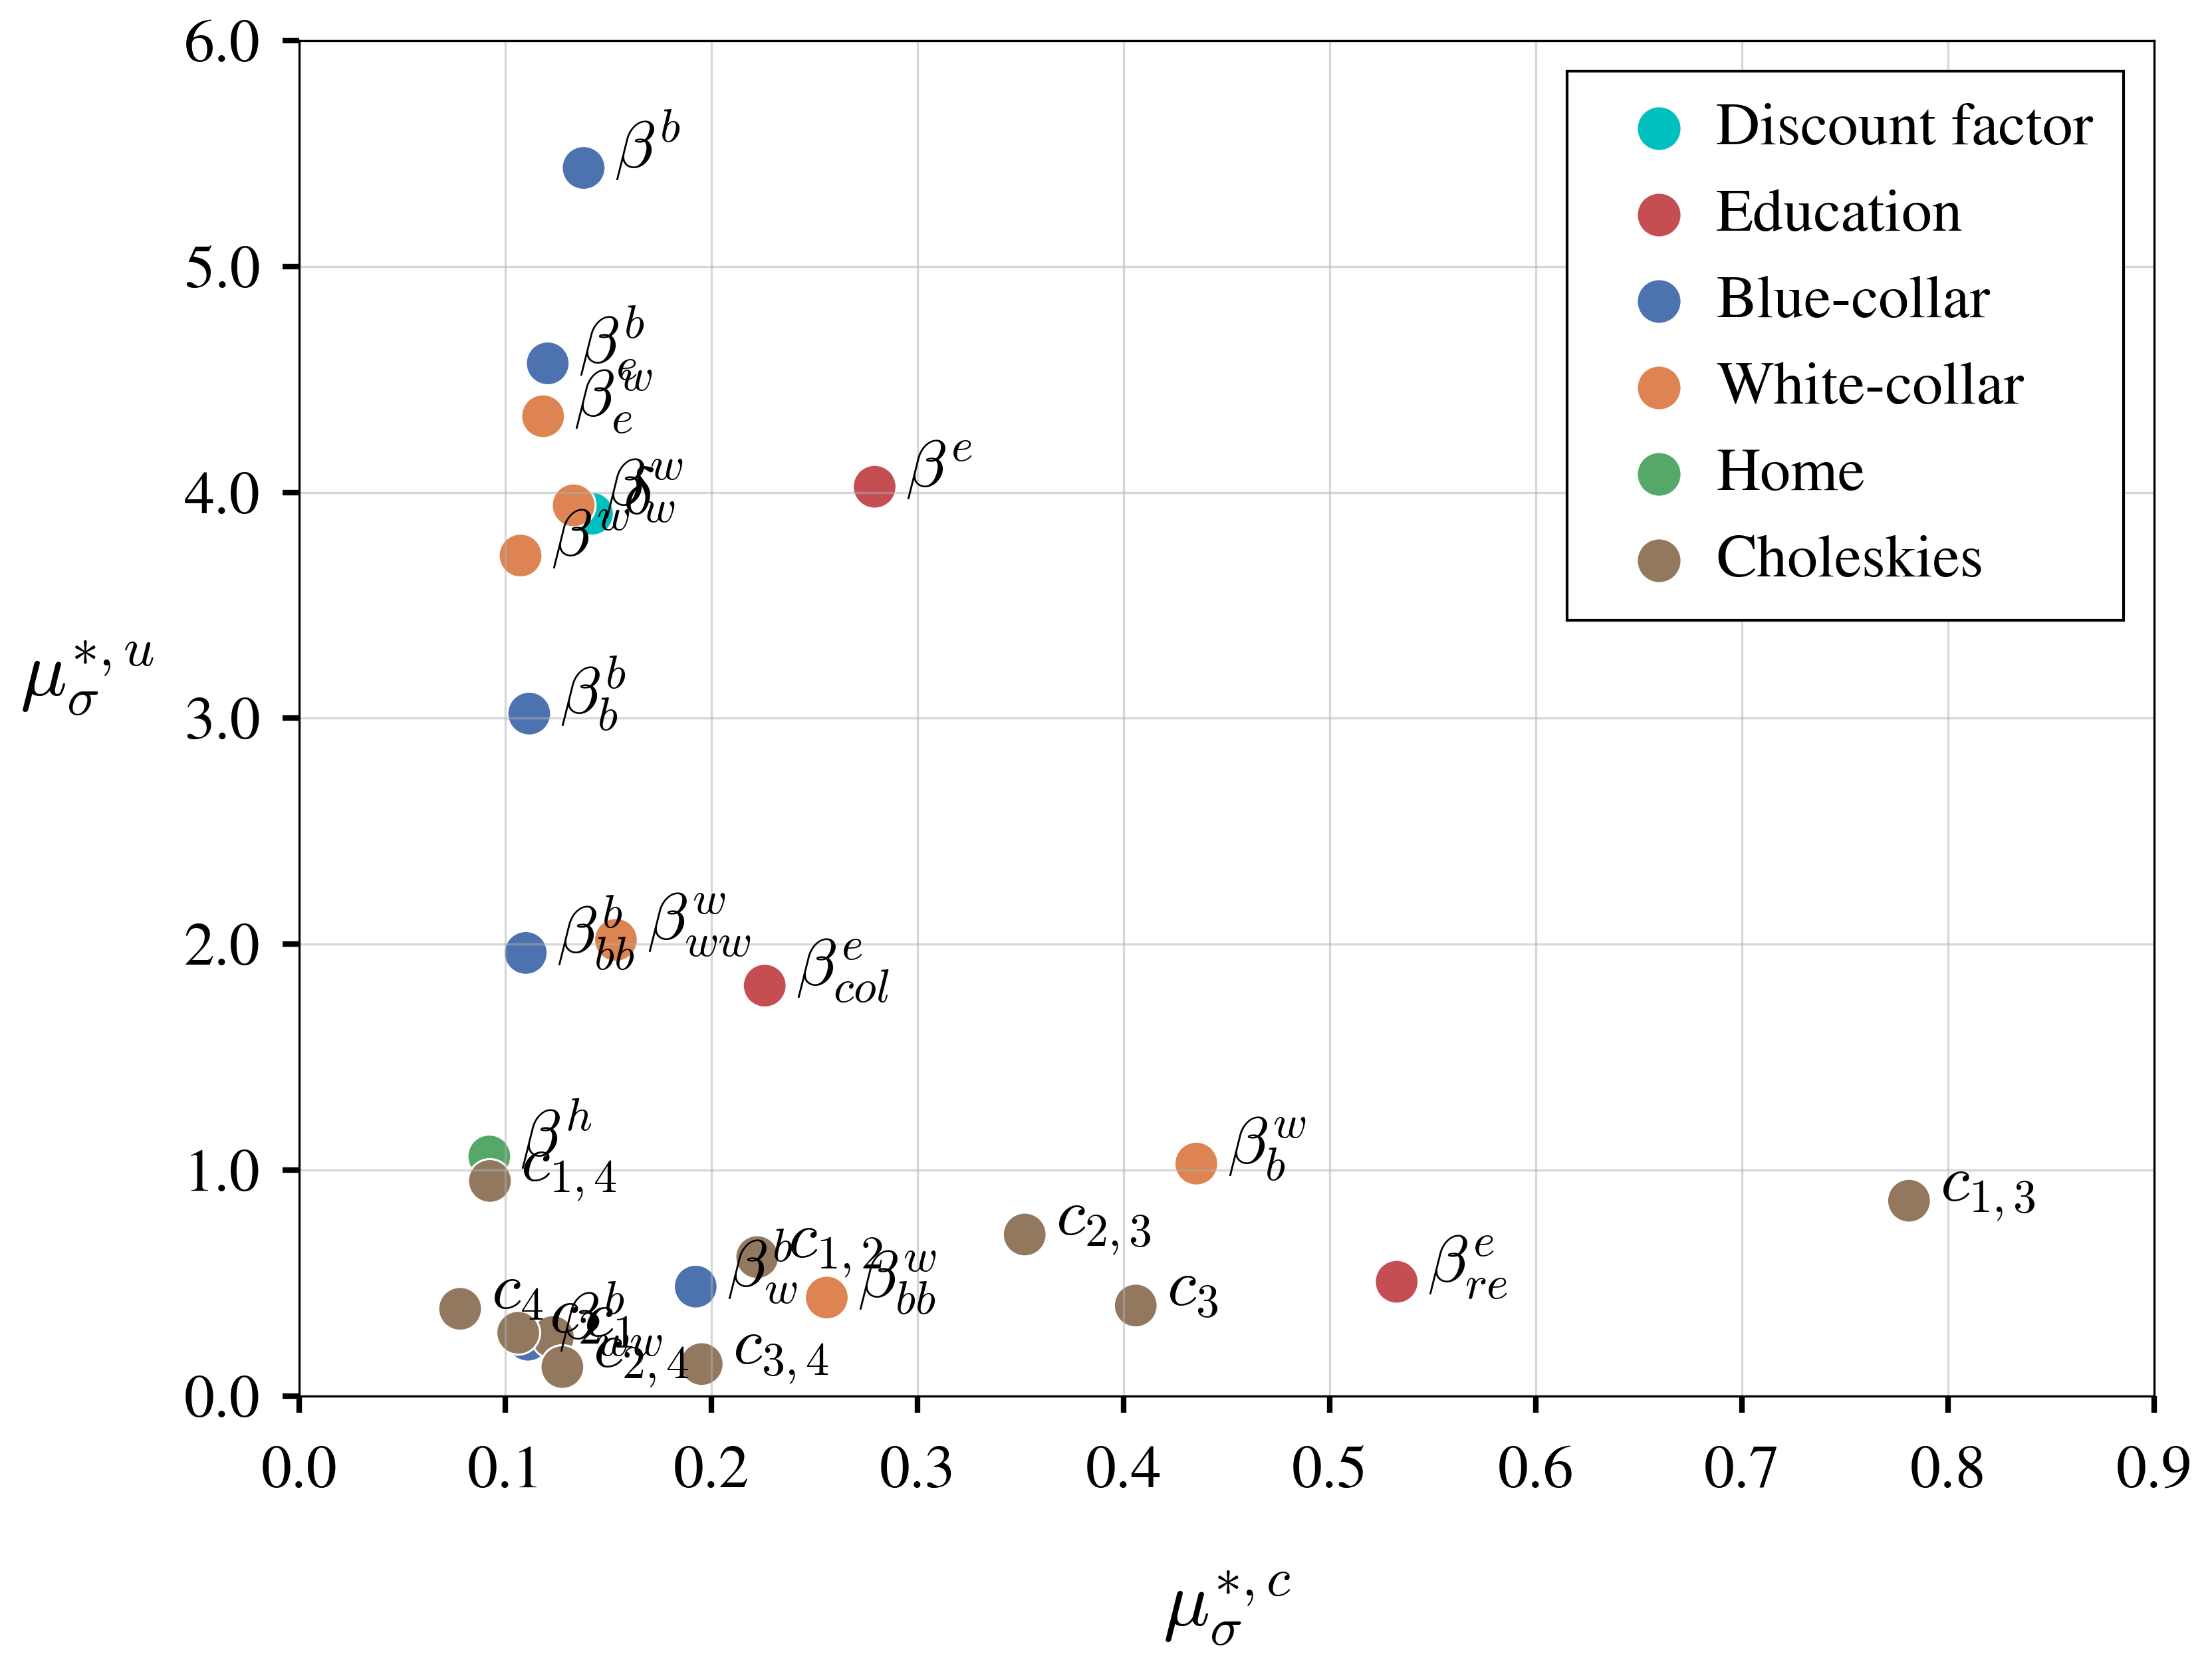
\includegraphics[scale=0.52]{../../../scrypy/figures/scatter_traj}
	\label{fig:traj}
\end{figure}

\begin{figure}[H]
	\caption{Sigma-normalized mean absolute Elementary Effects for radial design}
	\centering
	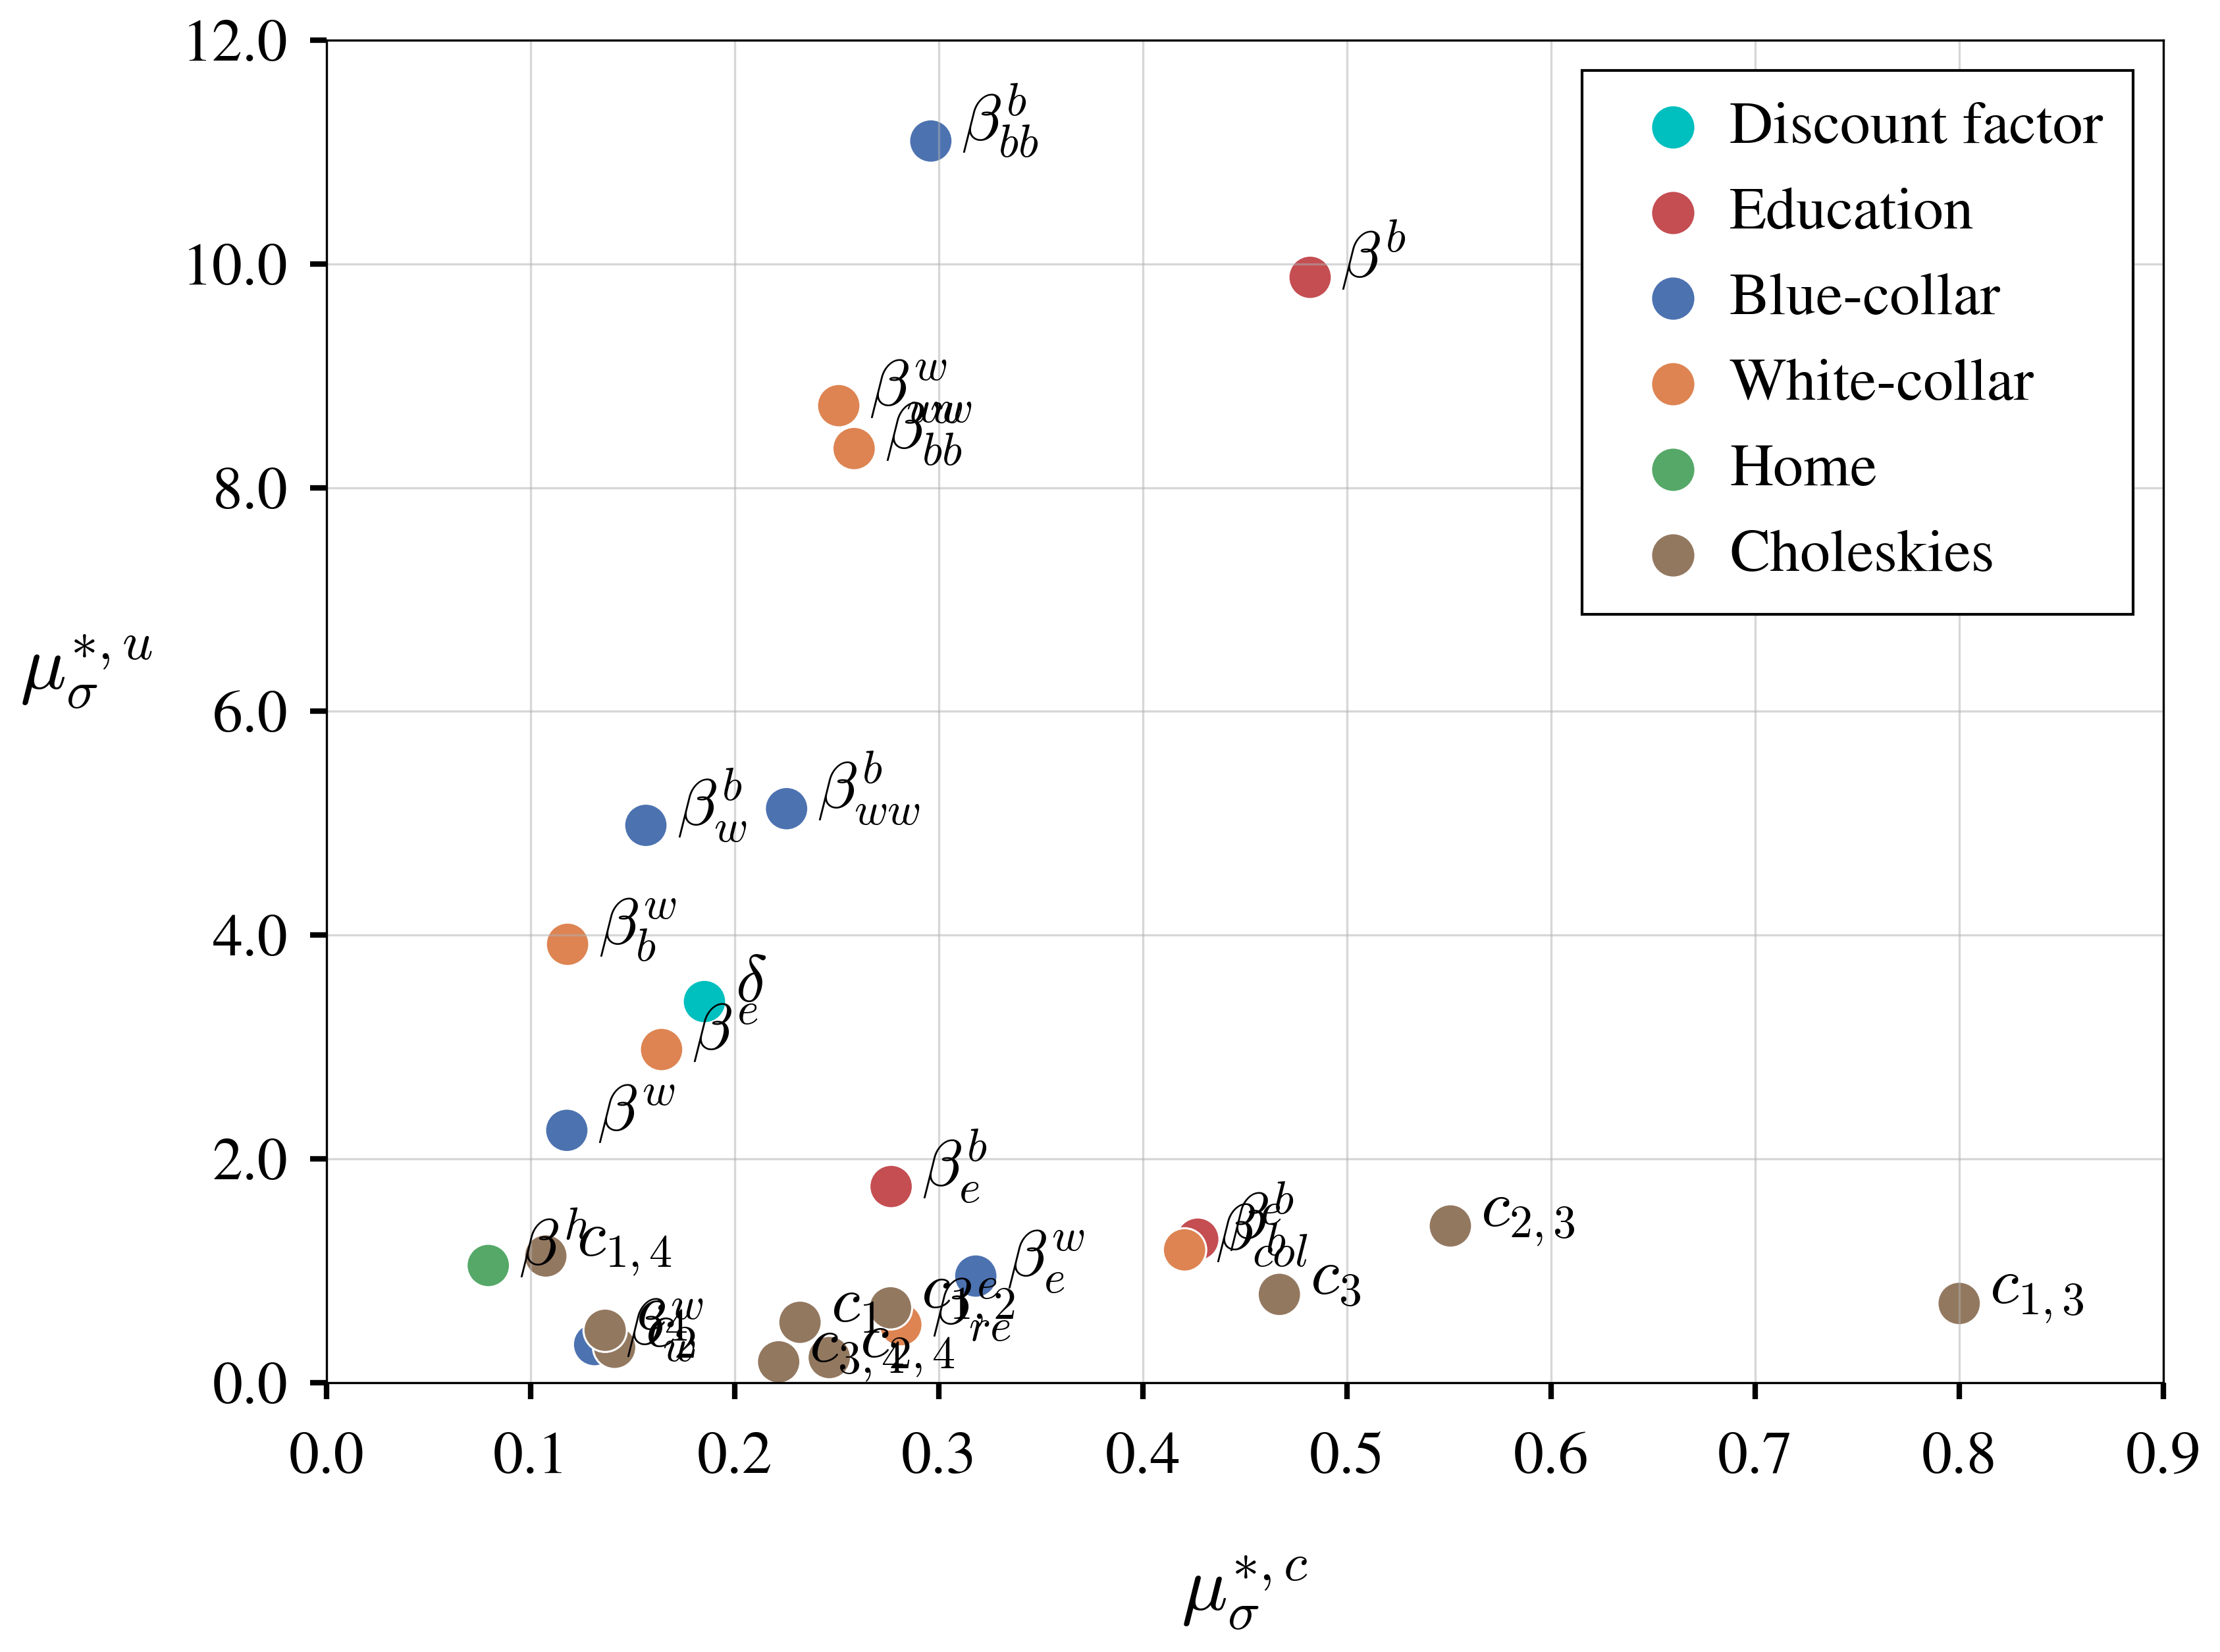
\includegraphics[scale=0.52]{../../../scrypy/figures/scatter_rad}
	\label{fig:rad}
\end{figure}


\newpage
\subsection{Review: Estimation Results}
% increase spacing between table columns
\setlength{\tabcolsep}{18pt} %from 6
\begin{table}[H] 
	\centering
	\begin{threeparttable}
		\caption[Model Parametrization]{Estimates for the distribution of input parameters}
		\label{tab:params}
		\renewcommand{\arraystretch}{1.2}%
		\begin{tabular}{cS[table-format=3.2]S[table-format=3.2]S[table-format=3.2]}
			\toprule
			{Parameter}     & {Mean}   & {Standard error (SE)} & {SE in KW94} \\ \midrule
			\textit{General} \\
			$\delta$ & 0.95   & 0.00084 & \textit{-}    \\    \midrule
			\textit{Blue-collar}\\    
			$\beta^b$ & 9.21   & .013            & 0.014      \\
			$\beta_e^b$ & 0.038  &    0.0011        & 0.0015       \\
			$\beta^b_b$ & 0.033  & 0.00044            & 0.00079       \\
			$\beta^b_{bb}$ & -0.0005 & 0.000013           & 0.000019       \\
			$\beta^b_w$ & 0.0    & 0.00067             & 0.0024      \\
			$\beta^b_{ww}$ & 0.0    & 0.000029           & 0.000096       \\ \midrule
			\textit{White-collar}\\
			$\beta^w$ & 8.48   & 0.0076             & 0.0123      \\
			$\beta^w_e$ & 0.07   & 0.00047          & 0.00096       \\
			$\beta^w_w$ & 0.067  & 0.00055            & 0.00090      \\
			$\beta^w_{ww}$ & -0.001  & 0.000017           & 0.000070     \\
			$\beta^w_b$ & 0.022  & 0.00033           & 0.0010      \\
			$\beta^w_{bb}$ & -0.0005 & 0.000021         & 0.000030      \\ \midrule
			\textit{Education} \\
			$\beta^e$     & 0.0    & 330                & 459       \\
			$\beta_{he}^e$     & 0.0    & 155               & 410       \\
			$\beta_{re}^e$     & -4000   & 202                & 660       \\ \midrule
			\textit{Home} \\
			$\beta^h$    & 17750  & 390                & 1442      \\ \midrule
			\multicolumn{4}{l}{\textit{Lower Triangular Cholesky Matrix}} \\
			$c_{1}$      & 0.2    & 0.0015             & 0.0056      \\
			$c_{2}$      & 0.25    & 0.0013             & 0.0046     \\
			$c_{3}$      & 1500   & 108             & 350      \\
			$c_{4}$      & 1500    & 173              & 786      \\
			$c_{1,2}$     & 0.0    & 0.0064              & 0.023     \\
			$c_{1,3}$      & 0.0   & 143               & 0.412      \\
			$c_{2,3}$      & 0.0    & 116             &  0.379     \\
			$c_{1,4}$      & 0.0    & 232             &   0.911    \\
			$c_{2,4}$      & 0.0    & 130            & 0.624      \\
			$c_{3,4}$      & 0.0   & 177                & 0.870       \\ \bottomrule
		\end{tabular}
	\end{threeparttable}
\end{table}
\subsection{Improvement: Sampling scheme tailored to Sobol' indices}

Similar to trajectory design to have interactions still included.
Base row is expectation. Shuffle row. Add random value between $[0, 0.5]$. Take square root of squared difference and divide by step.
\newpage
\bibliography{../../bibliography/literature}

\end{document}